\documentclass[10pt]{extarticle}
\title{}
\author{Avinash Iyer}
\date{}
\usepackage[shortlabels]{enumitem}

%font setup
%
\usepackage{newpxtext,eulerpx}

%paper setup
\usepackage{geometry}
\geometry{letterpaper, portrait, margin=1in}
\usepackage{fancyhdr}

%symbols
\usepackage{amsmath}
\usepackage{mathtools}
\usepackage{amssymb}
\usepackage{hyperref}
\usepackage{gensymb}

\usepackage[T1]{fontenc}
\usepackage[utf8]{inputenc}

%chemistry stuff
\usepackage[version=4]{mhchem}
\usepackage{chemfig}

%plotting
\usepackage{pgfplots}
\usepackage{tikz}
\tikzset{middleweight/.style={pos = 0.5, fill=white}}
\tikzset{weight/.style={pos = 0.5, fill = white}}
\tikzset{lateweight/.style={pos = 0.75, fill = white}}
\tikzset{earlyweight/.style={pos = 0.25, fill=white}}
%\usepackage{natbib}

%graphics stuff
\usepackage{graphicx}
\graphicspath{ {./images/} }
\usepackage{multicol}
%code stuff
%when using minted, make sure to add the -shell-escape flag
%you can use lstlisting if you don't want to use minted
%\usepackage{minted}
%\usemintedstyle{pastie}
%\newminted[javacode]{java}{frame=lines,framesep=2mm,linenos=true,fontsize=\footnotesize,tabsize=3,autogobble,}
%\newminted[cppcode]{cpp}{frame=lines,framesep=2mm,linenos=true,fontsize=\footnotesize,tabsize=3,autogobble,}

\usepackage{listings}
\usepackage{color}
\definecolor{dkgreen}{rgb}{0,0.6,0}
\definecolor{gray}{rgb}{0.5,0.5,0.5}
\definecolor{mauve}{rgb}{0.58,0,0.82}

\lstset{frame=tb,
	language=Java,
	aboveskip=3mm,
	belowskip=3mm,
	showstringspaces=false,
	columns=flexible,
	basicstyle={\small\ttfamily},
	numbers=none,
	numberstyle=\tiny\color{gray},
	keywordstyle=\color{blue},
	commentstyle=\color{dkgreen},
	stringstyle=\color{mauve},
	breaklines=true,
	breakatwhitespace=true,
	tabsize=3
}
% text + color boxes
\usepackage{tcolorbox}
\tcbuselibrary{breakable}
\newtcolorbox{problem}[1]{colback = white, title = {#1}, breakable}
\newtcolorbox{solution}{colback = white, colframe = black!75!white, title = Solution, breakable}
%including PDFs
\usepackage{pdfpages}
\setlength{\parindent}{0pt}

\pagestyle{fancy}
\fancyhf{}
\rhead{Avinash Iyer}
\lhead{Homework Section 2.3, Individual}
\begin{document}
  \begin{problem}{Dijkstra's Algorithm Modification}
    In class, we gave a version of Dijkstra's algorithm for finding the distance between a vertex $u$ and all the other vertices in a weighted graph. Appropriately modify that algorithm such that it not only outputs $d(u,v)$, but also outputs the shortest $u,v$ path.
    \tcblower
    We will commence the algorithm as follows:
    \begin{description}[font=\normalfont\scshape]
      \item[Input] A weighted graph, $G$, and $u\in V(G)$
      \item[Output] For each $z\in V(G)$, the distance $d(u,z)$, and the $u,v$-geodesic.
      \item[Initialization]Extend the weight function such that if $xy\notin E(G)$, then $w(xy) = \infty$. Create $S$ that contains all vertices whose distances from $u$ are known. Let $S := \{u\}$. Let $t:V\rightarrow \mathbb{R}^+ \cup \{0,\infty\}$ which will keep track of the tentative distance between $u$ and $z$. Let $t(z) := w(uz)$ for all $z\neq u$, and $t(u) := 0$. Additionally, create a path $P_{z}$ for $z$, starting at $u$ and ending at $z$. We will let $P'_{z}$ be the tentative path.
      \item[Condition to Terminate Loop] If $t(z) = \infty$ for all $z\notin S$ \textsc{or} $S = V$, then go to end.
      \item[Loop] Else, pick $v\in V-S$ such that $t(v) = \min_{z\notin S} t(z)$. Add $v$ to $S$. Explore the edges from $v$ to update tentative distances; for each edge $vz$ with $z\notin S$, $t(z) := \min\{t(z),t(v) + w(vz)\}$. Add $z$ to $P'_v$.
      \item[End] Set $d(u,v) = t(v)~\forall v\in V$, and set $P_v$ to $P'_v$ for all $v\in V$.
    \end{description}
  \end{problem}
  \begin{problem}{Modified Dijkstra's Algorithm, Example}
    Perform the modified Dijkstra's algorithm on the following graph:
    \begin{center}
      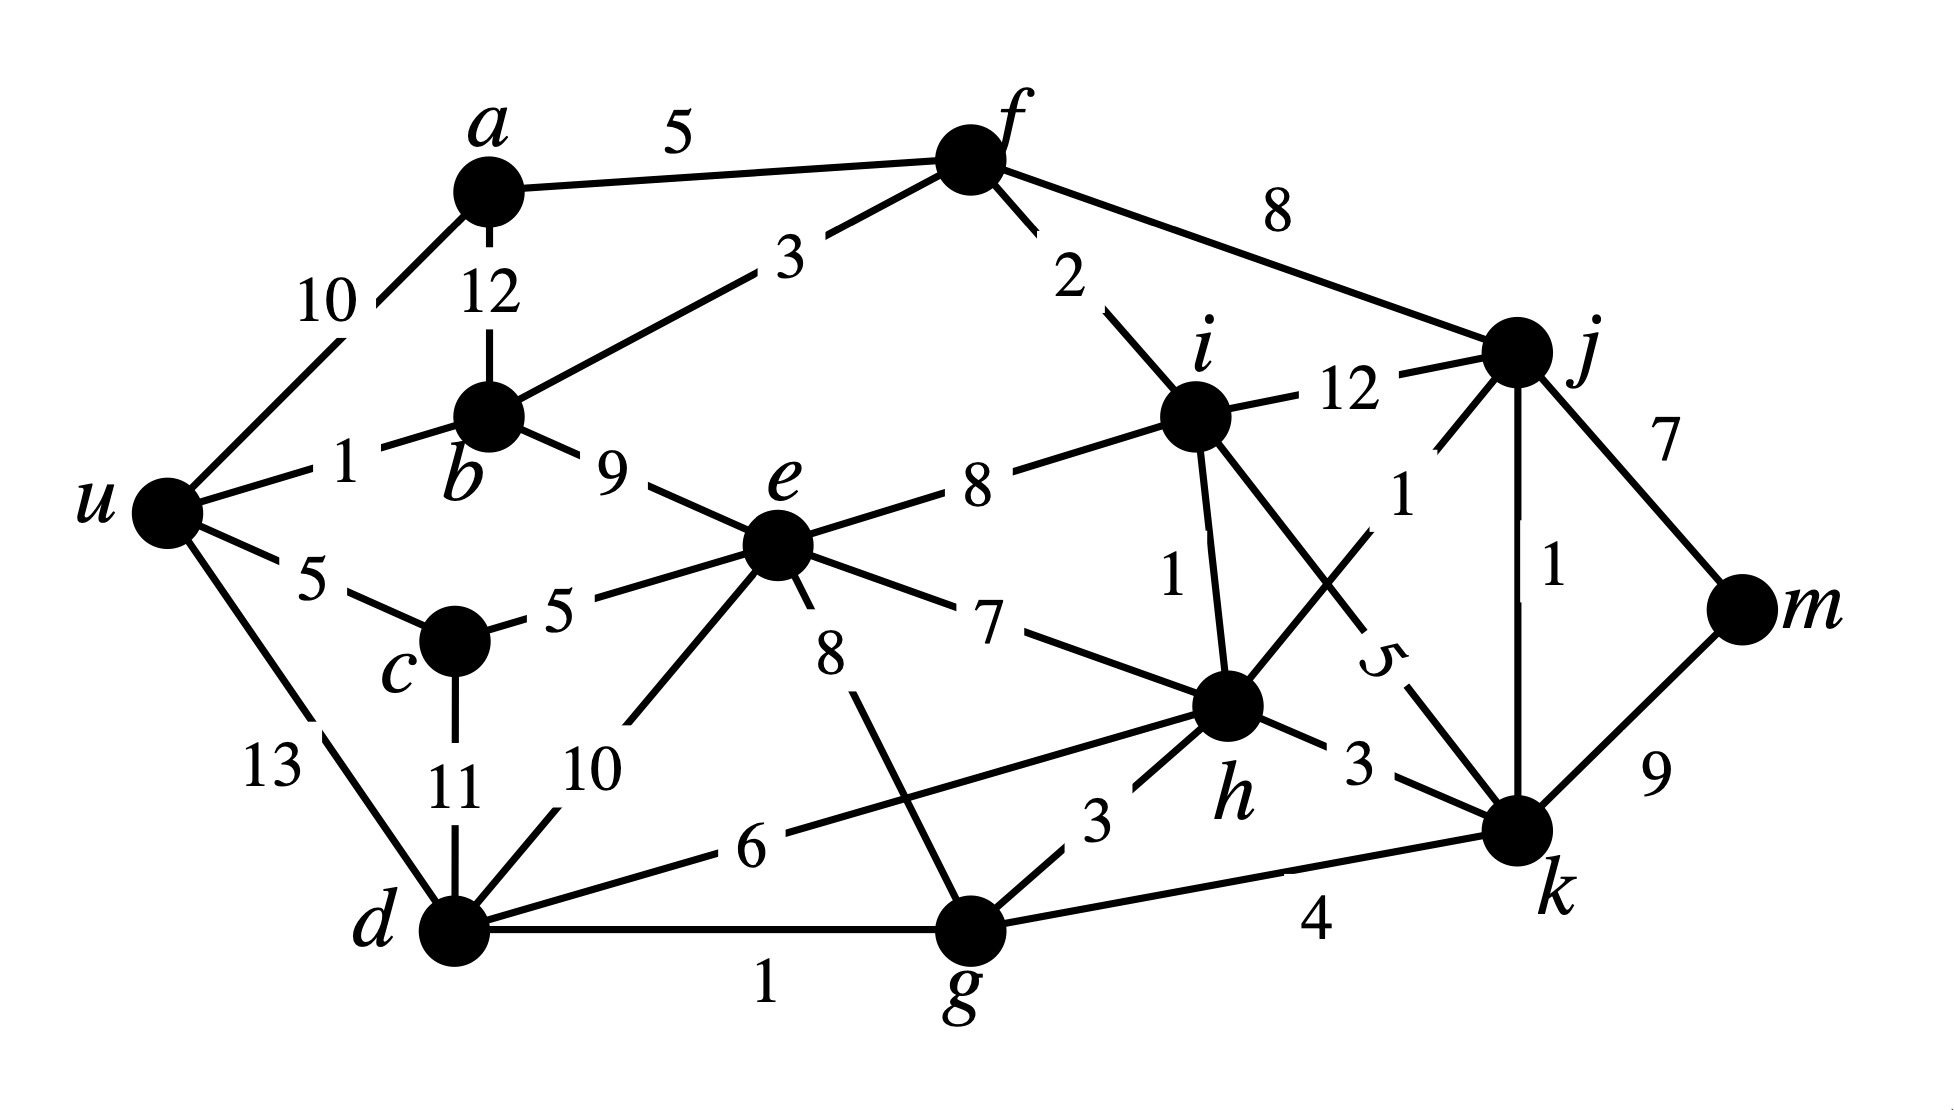
\includegraphics[width=10cm]{2_3_graph}
    \end{center}
    \tcblower
    \begin{center} 
      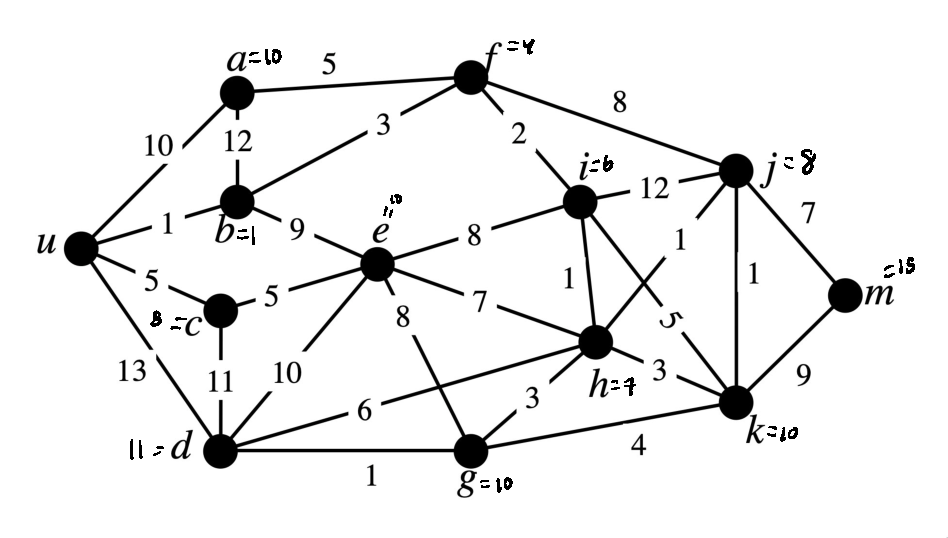
\includegraphics[width=10cm]{2_3_dijkstra}
    \end{center}
    Paths:
    \begin{multicols}{2}
    \begin{itemize}
      \item $P_a = u,a$
      \item $P_b = u,b$
      \item $P_c = u,c$
      \item $P_d = u,b,f,i,h,g,d$
      \item $P_e = u,b,e$
      \item $P_f = u,b,f$
      \item $P_g = u,b,f,i,h,g$
      \item $P_h = u,b,f,i,h$
      \item $P_i = u,b,f,i$
      \item $P_j = u,b,f,j$
      \item $P_k = u,b,f,j,k$
      \item $P_m = u,b,f,j,m$
    \end{itemize}
    \end{multicols}
  \end{problem}
  \begin{problem}{2.3.1}
    Assign integer weights to the edges of $K_n$. Prove that the total weight of every cycle in $K_n$ is even if and only if the total weight of each triangle is even.
    \tcblower
    \begin{description}[font=\normalfont\scshape]
      \item[$(\Rightarrow)$] Suppose there exists a triangle in $K_n$ whose weight is odd. Then, this triangle is a cycle in $K_n$ whose weight is odd, meaning that it is not the case that the total weight of every cycle in $K_n$ is odd.
      \item[$(\Leftarrow)$] Suppose toward contradiction that $K_n$ has a cycle of odd weight. Then, we will show that there exists a triangle of odd weight in $K_n$.
        \begin{description}[font = \normalfont\scshape]
          \item[Base Case:] If $n = 3$, then $K_n$ containing a cycle of odd weight means $K_3$, the triangle graph, is of odd weight, so $K_3$ contains a triangle of odd weight.
          \item[Inductive Hypothesis:] If $K_n$ contains a cycle of odd weight, then $K_{n-1}$ for some deleted vertex contains a cycle of odd weight, meaning that $K_{n-1}$ has a triangle of odd weight.
          \item[Proof:] For any cycle with odd weight, there must be an odd number of edges in the cycle of odd weight. Thus, for any vertex with an \textit{even} number of edges with odd weight incident on it, deletion maintains the parity of the total number of edges with odd weight. So, $K_{n-1}$ for the deleted vertex will still contain an odd cycle, and thus by the inductive hypothesis, $K_{n-1}$ will have a triangle of odd weight.
        \end{description}
    \end{description}
  \end{problem}
  \begin{problem}{2.3.2}
    Prove or disprove: If $T$ is a minimum weight spanning tree of a weighted graph $G$, then the $u,v$ path in $T$ is the minimum weight $u,v$ path in $G$.
    \tcblower
    This assertion is \textbf{false}, as we can see in the following graph:
    \begin{center}
      \begin{tikzpicture}
        \draw (0,0) -- node[weight]{1}(0,5) -- node[weight]{2} (5,5) -- node[weight]{3}(5,0) -- node[weight]{4} (0,0);
        \node[anchor = north east] at (0,0) {$a$};
        \node[anchor = south east] at (0,5) {$b$};
        \node[anchor = south west] at (5,5) {$c$};
        \node[anchor = north east] at (5,0) {$d$};
        \filldraw (0,0) circle (2pt)
                  (5,0) circle (2pt)
                  (5,5) circle (2pt)
                  (0,5) circle (2pt);
      \end{tikzpicture}
    \end{center}
    The minimum weight spanning tree is as follows:
    \begin{center}
      \begin{tikzpicture}
        \draw (0,0) -- node[weight]{1}(0,5) -- node[weight]{2} (5,5) -- node[weight]{3}(5,0);
        \node[anchor = north east] at (0,0) {$a$};
        \node[anchor = south east] at (0,5) {$b$};
        \node[anchor = south west] at (5,5) {$c$};
        \node[anchor = north east] at (5,0) {$d$};
        \filldraw (0,0) circle (2pt)
                  (5,0) circle (2pt)
                  (5,5) circle (2pt)
                  (0,5) circle (2pt);
      \end{tikzpicture}
    \end{center}
    But, we can see that the shortest weight path between $a$ and $d$ in $G$ is of weight $4$, while it is of weight $6$ in the minimum weight spanning tree.
  \end{problem}
  \begin{problem}{2.3.5}
    There are five cities in a network. The travel time for travelling directly from $i$ to $j$ is the entry $a_{i,j}$ in the matrix below. The matrix is not symmetric, and $a_{i,j} = \infty$ indicates there is no direct route. Determine the least travel time and quickest route for each pair $i,j$.
    \[
      \begin{pmatrix}
        0 & 10 & 20 & \infty & 17 \\
        7 & 0 & 5 & 22 & 33 \\
        14 & 13 & 0 & 15 & 27 \\
        30 & \infty & 17 & 0 & 10 \\
        \infty & 15 & 12 & 8 & 0
      \end{pmatrix}
    \]
    \tcblower
    Using Dijkstra's algorithm, we are able to find the optimal travel time as seen in the following table (where the column entry represents $i$ and the row entry represents $j$).
    \begin{center}
    \renewcommand{\arraystretch}{1.5}
      \begin{tabular}{c|ccccc}
        $(i,j)$ & 1 & 2 & 3 & 4 & 5 \\
        \hline
        1 & 0 & 10 & 15 & 25 & 17 \\
        2 & 7 & 0 & 5 & 14 & 24 \\
        3 & 14 & 13 & 0 & 15 & 25 \\
        4 & 30 & 25 & 17 & 0 & 17 \\
        5 & 22 & 15 & 12 & 8 & 0
      \end{tabular}
    \end{center}
  \end{problem}
  \begin{problem}{2.3.7}
    Let $G$ be a weighted connected graph with distinct edge weights. Without using Kruskal's algorithm, prove that $G$ has only one minimum weight spanning tree.
    \tcblower
    Let $E_{T} = \{e_1,\dots,e_k\}$ be the edge set of the minimum weight spanning tree of $T\subseteq G$. Suppose there exists a $T'$ such that $w(T')\leq w(T)$. Then, by the result from Exercise 2.1.37, we know that we can create $T'$ from $T$ by subtracting one edge in $G$ and adding a different edge in $G$, or that $T' = T-e+e'$.\\

    Since all the edges of $G$ are of distinct weight, then $w(e) \neq w(e')$, meaning that $w(T') \neq w(T)$. Therefore, it must be the case that the inequality is sharp, or that $w(T') < w(T)$ --- however, since we had assumed that $T$ was a minimum weight spanning tree, this means $T'$ cannot exist (or else it would be a minimum weight spanning tree), so there is only one minimum weight spanning tree in $G$.
  \end{problem}
  \begin{problem}{2.3.13}
    Let $T$ be a minimum weight spanning tree and let $T'$ be another spanning tree in $G$. Prove that $T'$ can be turned into $T$ by a list of steps that exchange one edge of $T'$ for one edge of $T$ such that the edge set is always a spanning tree and the total weight never increases.
    \tcblower
    Let $E(T')$ denote the edge list in $T'$ and let $E(T)$ denote the edge list in $T$. By Theorem 2.1.7, we know that for any edge $e'\in E(T') - E(T)$, there exists an edge $e\in E(T) - E(T')$ such that $T'+ e - e'$ is also a spanning tree of $G$. In the case where $T$ is a minimum weight spanning tree of $G$, we know that $T'$ must have a weight greater than or equal to $T$, and that any edge $e'$ that is exchanged for $e$, $w(e') \geq w(e)$. So, at the end of the program (where we have exchanged every $e'\in E(T') - E(T)$ for every $e\in E(T) - E(T')$), we know that any edge exchange must either reduce the total weight of $T'$ or keep the total weight the same.
  \end{problem}
\end{document}
